\begin{landscape}
\begin{figurels}[!]
    \centering
    \caption{Singles spectra of $^{154}$Gd. Spectra are labeled with the particles being detected, the energies of the $\gamma$ and electron spectra aligned for identification. In the $\gamma$ spectrum, several lines of note are labeled. The large peak at low energy in the electron spectrum is cut off due to the threshold. It is a combination of background and the 123K peak. Transitions in the higher energy regime of the $\gamma$ spectrum cannot be determined without gating, due to additional background from the experimental room. The electron detectors have a maximum energy of approximately 1250 keV, so there are no conversion electron spectra paired with the higher energy gamma spectra.}
    \label{fig:154Gd_Singles}
\end{figurels}
\begin{figurels}[!]
    \centering
    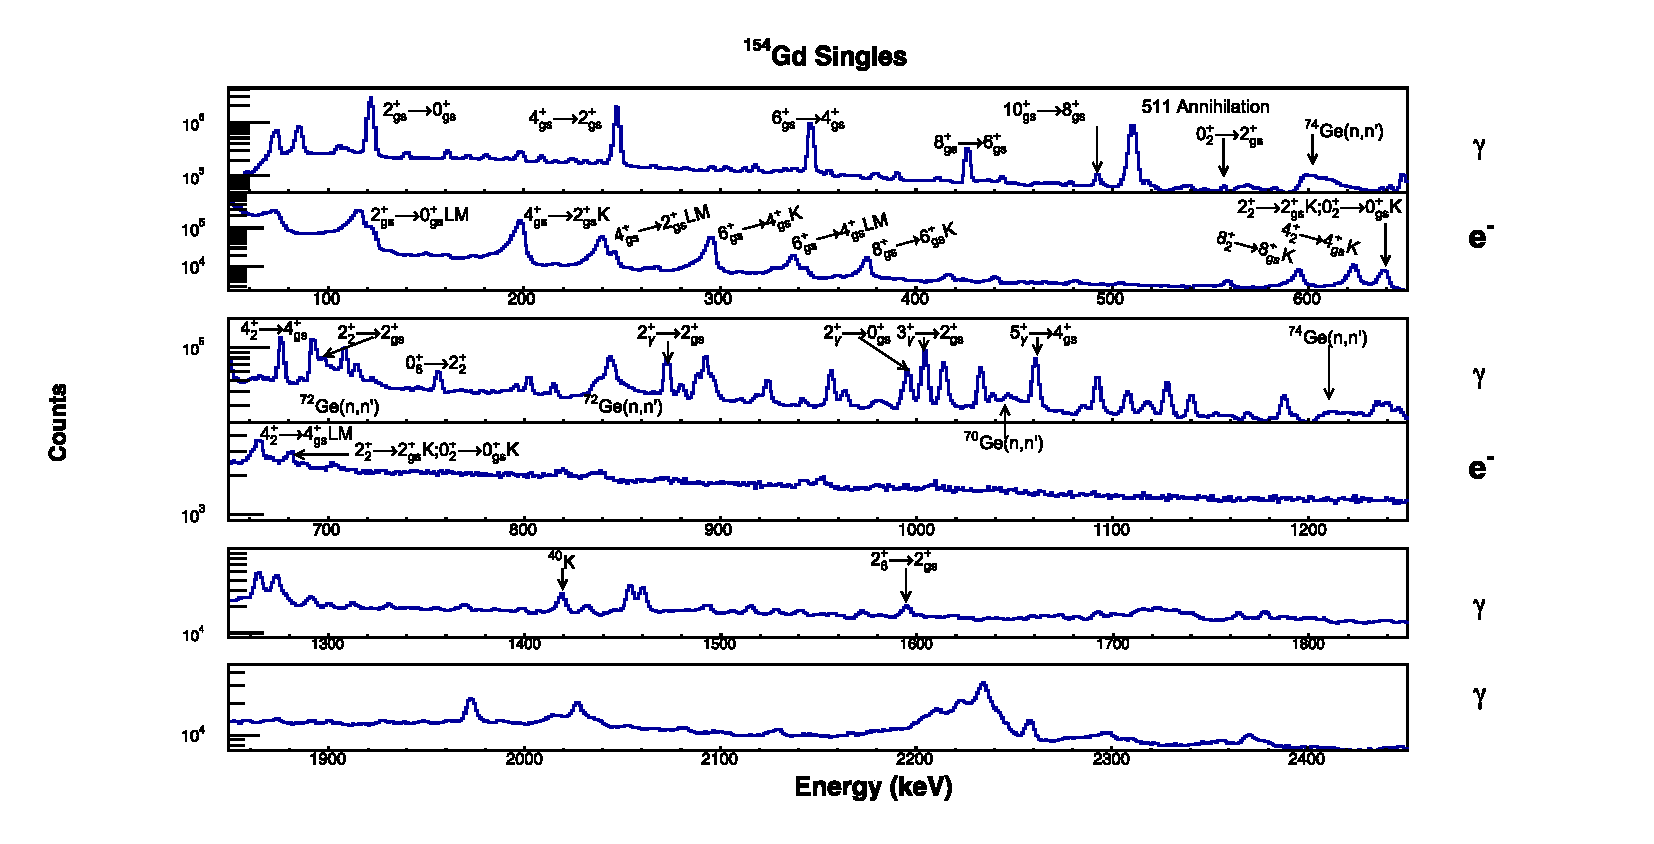
\includegraphics[scale=0.85]{154GdTablesAndFigs/154Gd_singles.eps}
\end{figurels}
\end{landscape}